\section{Introduction}
A player owes \$750 with \$168 in cash. Its response proposes selling one Boardwalk house, mortgaging Park Place and three other deeds, and leaving Boardwalk and Kentucky unmortgaged. Its actions carry out that selection and leave \$28. Another player values its entire portfolio at \$1,414, liquidates it to pay \$1,400, and retains the predicted \$14. The first assessment selects resources under financial slack; the second values a binding budget. Payment alone does not distinguish them.

Economic agency also requires considering other players' opportunities. Completing a group can enable construction; selling its buildings can enable mortgages; financing an opponent can prevent a stronger player from inheriting it. These relationships connect local financial decisions to strategic interaction. A language-model agent playing a complete game must operate within them while communicating, maintaining a portfolio and responding to consequences over many turns.

Monopoly offers a useful observational setting because monetary obligations, holdings and legal actions can be reconstructed. It also poses an interpretive problem. Winning combines decisions, opponents and chance, and completing a sequence through refreshed menus need not demonstrate a prior plan. Conversely, a written budget can expose a relevant dependency even when several reactive action orders would also succeed. Studying the relation between assessment and action therefore requires the delivered state, the agent's actual response and the executed continuation.

We study twenty complete games played by four configured LLM systems. The question is how their expressed economic assessments correspond to available resources, bargaining choices and applied actions. We examine every financing episode and offer response, then use eight selected incidents to explain particular tactics. The contributions are:
\begin{enumerate}
\item A complete financial census with verified feasibility categories and a structural account of what successful execution requires. It separates resource assessment and stopping from sequence completion.
\item An analysis of all sixteen obligations requiring newly available collateral, including both returned text channels, successful selective financing and the different recorded response patterns accompanying three payable declarations.
\item A complete negotiation census and contextual evidence of rival-development concerns, bargaining limits, selective disclosure and estate-related incentives, with proposer composition made explicit.
\end{enumerate}
The result is an observational account of economic conduct under the recorded configurations. It is not a model ranking. Appendix~\ref{app:questions} maps the evidence to broader questions about strategy, memory, learning and multi-agent capability, distinguishing those this cohort can address from those it cannot.

\section{Study design}
\label{sec:setup}
\subsection{Game, information and response contract}
Four players begin with \$1,500 on the US Monopoly board. They buy, auction, trade and develop properties, with bilateral negotiations allowing up to twenty exchanges. The rules engine produces legal action menus and applies valid structured tool calls. It refreshes the financing menu after every sale or mortgage and automatically pays the current obligation once cash suffices. The financing instruction permits bankruptcy when the player ``cannot or should not raise enough cash.'' Thus declaring is allowed even when payment is possible.

The implementation retains the familiar rule that buildings must be removed before the group's deeds become mortgageable. It also differs from the published rules~\cite{hasbroMonopolyRules}: buildings pass intact to a player-creditor, inherited mortgages incur no immediate interest, and hotel-sale availability depends on bank house stock. These variants are not enumerated in the system prompt. Rules and the historical feasibility checks are documented in Appendix~\ref{app:rules}; inference about an agent's financial beliefs must use the rules it could have understood as well as those actually enforced.

Requests contain current cash, holdings, buildings, mortgages and bank stock, a twenty-entry public timeline, up to ten own notes, and the current legal menu. Trade responses also receive the proposed terms. Purchase prompts show board prices and rents; liquidation and trade states identify deeds by key without their financial values. Earlier notes and timeline entries can contain those values. The prompt permits bluffing and deception in public communication and requests honest private notes. Such conduct is authorized play, not evidence of unprompted misalignment.

A private note is an argument in the same tool call as the selected action. Assistant content is separate prose accompanying that call. The gateway can also return a readable reasoning field, labeled as a summary for Sol and Grok and as reasoning text for Gemini and Opus. We call it the \emph{returned explanation}; its completeness is unknown. These fields can disagree. A valid received call determines the applied action. Neither the note's position in JSON nor an explanation accompanying the action establishes an independent forecast or the model's internal computational order~\cite{turpin2023unfaithful,lanham2023faithfulness}.

\subsection{Cohort and configuration}
Five seeds each have four cyclic seat rotations of one roster. Every system occupies each seat five times but always follows the same opponent. The games last 75--386 turns and end with three eliminations. There are 6,989 decisions, 8,679 attempts and 50,918 events. System wins are 8/7/3/2 for Sol/Gemini/Opus/Grok; seat wins are 7/7/3/3. The repeated seeds do not hold later random exposure fixed when actions diverge.

\begin{table}[t]\centering\small
\begin{tabularx}{\linewidth}{@{}lYr@{}}\toprule
Label & OpenRouter identifier & Decisions\\\midrule
Sol & \path{openai/gpt-6.1-sol}&1,961\\
Gemini & \path{google/gemini-4-argon}&1,669\\
Opus & \path{anthropic/claude-opus-5.5}&1,696\\
Grok & \path{x-ai/grok-4.7}&1,663\\\bottomrule
\end{tabularx}
\caption{The four evaluated configurations. Requests specify medium reasoning effort, without a common token cap. This setting does not equalize provider-reported reasoning tokens.}
\end{table}

Two conditions are consequential. Opus produces 1,604 first-attempt refusals and one later refusal with an identical provider message about reverse engineering or duplicating outputs. Recovery drops the private-note request, retains permission to deceive and is never refused in 1,604 uses. Every first attempt in G5--G20 is refused; the transition occurs within the collection afternoon, already during G1--G4. Opus usually acts without an authored note and has no remaining corrective retry. It still receives public history and state.

Grok uses required tool choice while the others use automatic choice, confirmed in all 8,687 saved outgoing requests. In 139 responses its call names a different action from its assistant content, including 64 of 136 thread openings and seven of 28 acceptances. These settings are not experimentally separated from model identity. A formatter also misattributes past trade summaries in 2,054 initial prompts; current holdings and all 920 delivered offers agree with the legal acceptance menus. Appendix~\ref{app:prompts} gives prompts, recovery behavior, token accounting and recorded cost. These are the systems studied, not interchangeable deployments of four underlying models.

\subsection{Analysis populations}
A financing episode begins when cash is insufficient and the engine requests explicit financing. Let debt be $D$, cash $C$, total building salvage $S$, initially offered mortgage principal $M_0$, and all unmortgaged owned principal $M_*$. Define
\[
U_0=C+S+M_0,\qquad U_*=C+S+M_*.
\]
If $U_*<D$, even nominal own resources cannot pay. If $U_0<D\leq U_*$, a payment route must use mortgages absent initially. An upper bound alone is not a route: actual payments and retained engine-checked sequences establish feasibility, and source arguments justify the resource partition.

An offer is a set of terms awaiting a response. A counter changes its author; it need not change the thread's initiator. Completion refers to newly owning every deed in a color group, including mortgaged deeds. We separate stage, offer form, proposer and recipient. All contrasts and incidents are retrospective. Game and seed-block resampling describe uncertainty conditional on this selected corpus; they neither correct the selection of hypotheses nor create independent replications. Semantic readings are model-assisted, not human-validated. Exact fields, channels and case definitions accompany the data.

\section{Financial assessment and the decision to continue}
\label{sec:execution}
\subsection{What the complete census establishes}
Of 188 financing episodes, 128 end in payment and sixty in elimination. Payment uses 180 mortgages and 89 sale actions to meet \$51,997 in obligations. Sixty-seven payments take one action; sixty-one take two to ten. No successful episode uses an engine fallback. Three declared positions are also payable. Fifty-six other eliminations have $U_*<D$; in the last, G7 Opus, nominal resources of \$1,310 exceed a \$750 debt but only \$440 is accessible through the supplied menu.

\begin{table}[t]\centering\small
\begin{tabularx}{\linewidth}{@{}Yrr@{}}\toprule
Requirements of payable episodes & N & Paid\\\midrule
Cash and initially listed mortgages suffice &62&62\\
Sales required; released mortgages unnecessary &53&52\\
Released mortgages necessary &16&14\\\midrule
All demonstrated-payable episodes &131&128\\\bottomrule
\end{tabularx}
\caption{Financing requirements, not measured planning difficulty. Appendix~\ref{app:finance} explains the sufficiency evidence for each category.}\label{tab:debt-requirements}
\end{table}

The menu provides substantial assistance. For all 131 historical payable entries, source analysis shows that an uninterrupted sequence of valid, strictly cash-raising sales or mortgages must eventually pay if the player does not declare. Before payment, cash plus remaining salvage and mortgage principal is invariant; each action reduces a finite stock of financing resources. Recorded ownership, development and bank-stock conditions prevent an unpaid dead end. Appendix~\ref{app:continuation} gives the proof and its coverage, including the two hotel-stock cases requiring a separate argument. This is a source-based result, not a measured policy run, and excludes invalid calls, exhausted call budgets and later obligations.

Consequently, 128 payments do not demonstrate that agents solved difficult action-order problems. They establish realized financing under an assisting interface. The more discriminating observations are their financial inventories, decisions to stop, selected assets and agreement between text and calls.

Asset selection shows a consistent preference in one defined population. Of the 62 episodes payable from cash and initially listed mortgages, thirty debtors own buildings. Twenty-eight pay without selling any; the other two, both Opus, sell one house each. These choices preserve development when mortgages already provide sufficient financing. They describe the assets retained, without establishing that the chosen route minimizes cost or maximizes future income.

\subsection{Resources beyond the initial menu}
For each necessity episode, we classify the authored note when present and otherwise the returned explanation: eleven notes and five Opus explanations. Table~\ref{tab:text-types} describes these selected fields, rather than the strongest statement across every channel. Five successful fields explicitly state the release dependency, three order sales before using released collateral, five include that collateral in a budget, and one raises it tentatively. Both failures omit the resource from a claimed maximum. Appendix~\ref{app:finance} defines the categories, and all other available channels remain printed alongside each selected field.

\begin{table}[t]\centering\small
\begin{tabularx}{\linewidth}{@{}Yr@{}}\toprule
Selected field's expressed evidence & N\\\midrule
Explicit dependency between sale and mortgage &5\\
Ordered route using released collateral &3\\
Inclusive budget without explicit dependency &5\\
Tentative released-resource calculation &1\\
Incomplete inventory followed by declaration &2\\\bottomrule
\end{tabularx}
\caption{Model-assisted readings of one selected field per first resolved response. The first four categories end in payment; the last ends in bankruptcy. These labels do not certify every assertion in the field.}\label{tab:text-types}
\end{table}

\begin{figure*}[t]\centering
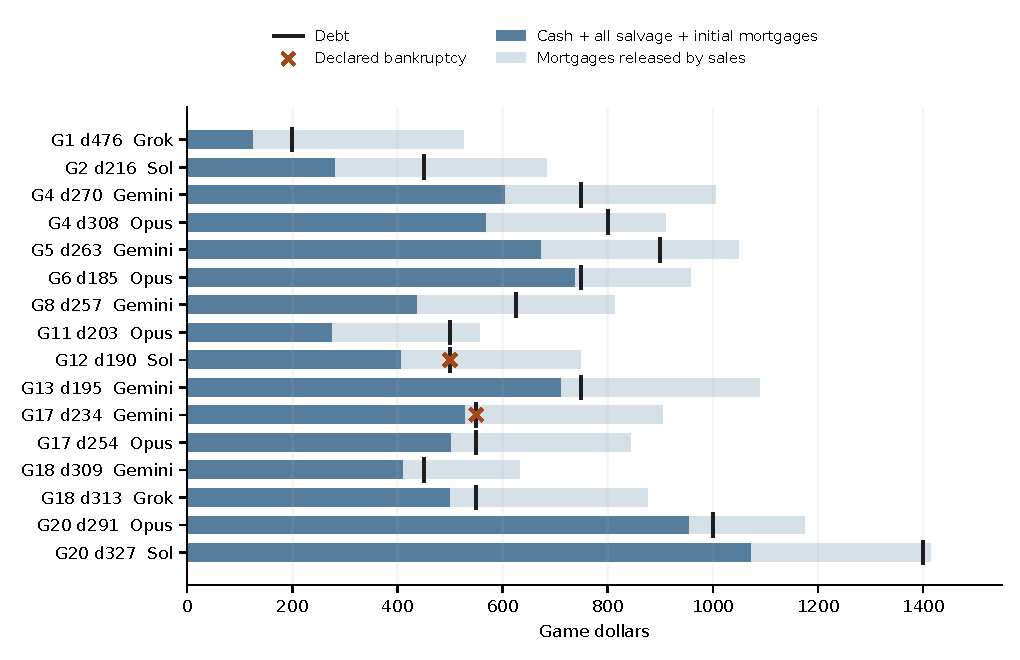
\includegraphics[width=.88\textwidth]{financial_dependencies.pdf}
\caption{The sixteen obligations requiring collateral absent from the initial mortgage menu. Dark bars add cash, all building salvage and initially listed mortgages; pale extensions add the released collateral. Debt exceeds the dark bar in every case. Crosses identify the two declarations. These resource sums establish necessity, while actual routes or retained legal sequences establish payment feasibility.}\label{fig:finance}
\end{figure*}

The successful responses apply familiar Monopoly knowledge to the current portfolio. For example, Gemini in G13 d195 starts with \$168 against \$750 owed. Its note specifies selling Boardwalk's house for \$100, mortgaging Park Place for \$175 and three other deeds for \$335 while leaving Boardwalk and Kentucky unmortgaged. The applied sequence follows that selection and leaves \$28. This is a concrete asset-preservation preference and sufficient route, without a claim that it minimizes cost or maximizes future winning chances.

Successful assessment is not uniformly exact. Sol's G2 d216 note values the yellow mortgages at \$430 rather than \$400 but still gives a sufficient route. Opus's G20 d291 explanation tentatively considers the pink mortgages with muddled intermediate arithmetic; the executed sequence pays and leaves \$25. Several statements compute maximum resources while the action sequence stops after raising less. Those distinctions matter when interpreting a text as a plan.

\paragraph{Incident 1: exact valuation across a long sequence.}
In G20 d327 Sol faces \$1,400 rent with \$49 cash, nine orange houses and two brown hotels. Its private note states the \$1,414 total and \$14 remainder. Its returned explanation supplies components totaling \$700 salvage and \$665 mortgage principal; the events realize those proceeds through two bundled sales and eight mortgages. Gemini had independently stated the same total before setting the rent, though its component errors offset by \$25. Because the smallest remaining asset increment exceeds \$14, full liquidation is forced if Sol pays; ten actions do not imply ten difficult route choices. The evidence is exact portfolio valuation, a stated target and its realization through feedback. The full notes appear in Appendix~\ref{app:casebook}.

The two failures make a different decision using a precise but incomplete inventory. Sol in G12 d190 adds \$53 cash, \$225 salvage and \$130 listed mortgages, obtaining \$408 against \$500 owed. It omits \$340 released red mortgages. Gemini in G17 d234 adds \$500 salvage and \$30 listed mortgages against \$550 owed, omitting \$375 released dark-blue mortgages. Both declare immediately. Their addition is correct. Their statements of available resources are not exhaustive.

Other channels complicate the interpretation without changing those omissions. Sol's returned explanation additionally considers property transfer through bankruptcy. Gemini's ends by mentioning further options. A private note and selected action are jointly emitted, and returned explanations can be incomplete. We therefore identify false financial assessments and their accompanying declarations, not a proven internal cause of surrender. The original instruction also permits surrender for strategic reasons.

The same two systems succeed elsewhere: Sol pays two of its three necessity episodes and Gemini five of six. In G5, Gemini's returned explanation revises a salvage-only subtotal to include dark-blue mortgages, then its note and payments realize a \$1,049 budget and \$149 remainder. Carried notes contain conditional mortgage inventories before four successes as well as the two failures. The repeated \$130 and \$30 figures in failed sums are true values of initially listed mortgages; their recurrence alone does not establish harmful memory anchoring.

\subsection{Stopping, continuing and conflicting responses}
The third payable declaration, G12 Grok d249, is not an omitted-resource case. Grok's note recognizes a sale-based route and its assistant content names a sale, while its received tool call declares. The legal route would pay the \$250 debt by selling five pink houses. Distinguishing a false budget from a conflicting response preserves their different implications for agent design.

The converse cases also matter. Six above-bound episodes start financing rather than declaring immediately. Five are Grok calls that conflict with the declaration named elsewhere in the response. In the sixth, G18 Gemini d344 mortgages to impose a ten-percent transfer fee on its creditor. That fee belongs to the published rulebook but is absent from this implementation. This is a rule mismatch in a stated strategic motive, not simply incorrect recollection. All six are documented alongside the payable declaration in Appendix~\ref{app:divergences}. A broader scan finds nine named-action conflicts in 338 liquidation decisions, all Grok, but explicit action naming is much more observable in Grok's content; it is not an equivalent conflict-rate comparison across systems.

\section{Bargaining over another player's opportunities}
\label{sec:bargaining}
\subsection{The complete response population}
The 526 threads contain 113 acceptances, 394 counters and 413 rejections. Acceptance is legal in 918 of 920 response opportunities. Sol and Opus counter in 140/235 and 141/189 responses; Gemini and Grok reject in 180/242 and 149/254. Each accepts 26--30 offers. Similar agreement totals therefore coexist with very different response styles.

Opening swaps completing only the proposer receive 95/116 rejections, compared with 37/72 completing neither player. Grok authors 36 of the 72 neither-completing swaps and fifteen of that cell's seventeen acceptances, but only eight of the 116 proposer-only swaps. Thirteen of those fifteen accepted Grok offers originate in calls whose content names another action. Removing Grok-authored offers changes the 30.5-point gap to 16.7 points, with game/block bootstrap percentile intervals including zero. This is an exploratory association among non-equivalent offers, not an identified response to completion.

\begin{table}[t]\centering\small
\begin{tabular}{@{}lrr@{}}\toprule
Opening offers & Proposer only & Neither\\\midrule
Swaps, all proposers &95/116&37/72\\
Swaps, excluding Grok &90/108&24/36\\
Cash bids, all proposers &42/70&67/103\\\bottomrule
\end{tabular}
\caption{Rejected/received in the exploratory comparison. The full form-by-completion population, proposer and recipient strata, block counts and bootstrap schemes are in Appendix~\ref{app:comparisons}.}
\end{table}

Pure cash bids show a pooled difference of $-5.0$ points; within-recipient differences range from $-0.2$ to $+8.5$. Opus authors 110 of these 173 cash bids, so the forms also differ in proposer composition. Later swaps are selected by preceding bargaining. None of these cuts isolates how a particular player would respond if only the rival's future opportunity changed.

Statements provide a separate source of evidence. Two Astra readings agree on explicit trade-linked rival consequences in 61 of 74 legally acceptable recipient-completing refusals: 27/38 recipient-only and 34/36 both-completing. This population is disjoint from the proposer-only/neither comparison. It documents the considerations agents express, not a semantic explanation of that contrast.

\subsection{Development, blocking and asking prices}
\paragraph{Incident 2: declining one's own monopoly.}
In G15, Sol offers two greens for Grok's Ventnor and \$100, completing both groups. Grok refuses while citing Sol's resulting yellow development and its own lack of green-building reserves. Two improved offers also fail. Grok had recorded its blocking policy thirty turns earlier, before a delivered public warning from Opus. The later refusals thus follow an existing policy; the warning cannot be credited with persuading it. Grok's blockers eventually pass to Gemini through bankruptcy, and Sol never completes either group. The case establishes expressed concern about relative consequences, not the optimality of refusal.

\paragraph{Incident 3: pricing control of yellow.}
In G2, Sol asks non-completer Grok \$450 for Marvin Gardens, then asks completing buyer Opus \$650. Opus publicly calls \$450 final while retaining a \$475 private ceiling; no trade settles. Sol had already stated a blocking policy before Grok publicly warned against the sale. Its estimate of Opus's building capacity overstates what \$520 buys, illustrating why attention to development and accurate valuation must be distinguished. Later, cash-poor Opus sells its two yellows to Sol. Sol develops and then liquidates them, receives \$44 undeveloped rent but no developed yellow rent, and loses them to Gemini. An apparent completion opportunity is only one stage of a longer financing history.

Prices cannot be reduced to a stable completion premium in this cohort. Six same-game, same-seller, same-deed comparisons retain mortgage status: four ask more of the completing buyer, one less and one the same. The seventh changes mortgage status. Countering also commonly preserves the exchange: 79/111 counters to proposer-only completion improve the counterer's cash without changing noncash terms, versus 81/110 non-completing deed requests. Ordinary repricing and completion-related considerations coexist.

\paragraph{Incident 4: a settled bargaining-limit bluff.}
In G7, Grok publicly offers ``\$600, final'' for North Carolina while its private note retains willingness to accept Sol's \$625. Sol settles at \$600. This directly juxtaposes a public limit with a higher private contingency under a prompt allowing deception. Later, Sol asks \$700 for New York to fund its dark blues. Gemini counters at \$520, explicitly calculating Sol's remaining development cost; Sol maintains its ask after noting that Gemini can mortgage other deeds to fund oranges. Gemini pays \$700, mortgages five deeds and builds four orange houses. The bargain involves stated assessments of both parties' subsequent financing, beyond the fact of agreement.

\subsection{Survival and inheritance as bargaining objects}
\paragraph{Incident 5: selling financial insurance.}
In G13, Grok asks Opus \$200 for mortgaged Pennsylvania, presenting the cash as necessary to avoid bankruptcy on a forthcoming railroad landing and keep yellows out of Sol's estate. Opus counters at \$130. Grok's returned explanation explicitly says it will omit a Ventnor mortgage that could make \$130 sufficient. Opus accepts \$200, while its own explanation weighs both denying Sol the yellows and potentially inheriting them itself. The buyer already considers that estate logic before the omission-framed reply. The record shows selective presentation and estate-based bargaining, without identifying whether the omission caused the extra \$70. Grok misses the immediate railroad landing and eventually loses the yellows to Sol; Opus later wins. The pitch's landing probability is inaccurate and is preserved as quoted evidence, not endorsed arithmetic.

Three further incidents complete the casebook. In G19, Sol corrects the false claim that States Avenue belongs to orange, yet accepts the economic terms. In G20, Gemini calls for denying Grok development finance and later refuses a purchase; another player continues offering funds, so the appeal is not evidence of collective compliance. In G18, Opus renews a standing offer while its returned explanation already expresses concern about prolonging Sol's survival, then withdraws when Sol invokes it. These are distinct acts: correction, attempted coordination and a contingent assurance. Their chronology and complete source-linked quotations appear in Appendix~\ref{app:casebook}.

The stakes are persistent. Thirty-eight of forty nonterminal eliminations follow rent on the creditor's developed color property. Those estates transfer 227 deeds and complete 52 groups during play. Buildings and future ownership therefore give the observed bargaining arguments economic content. These counts describe the pathway through which positions change; they do not identify the causal contribution of a tactic to winning.

\section{Relation to prior work and implications}
AgentMonopoly studies behavioral patterns and persona control, while FinBoardBench evaluates finance across several games and includes a sell-or-mortgage phase~\cite{wu2026agentmonopoly,hu2026finboardbench}. Multi-step financing is therefore not unique to this environment. Vending-Bench studies economic operation over long horizons, and Cattle Trade and DECE examine strategic interaction in other games~\cite{backlund2025vendingbench,muller2026cattletrade,zhang2026dece}. Our contribution is a complete account of encountered financing and negotiation, connecting expressed consequences to local financial ground truth and subsequent action under recorded response conditions.

PlanBench and ACPBench already study planning and action reachability, and PlanBench's o1 evaluation includes false impossibility judgments~\cite{valmeekam2023planbench,kokel2025acp,valmeekam2024o1}. Those constructs are not new here. The structural financing argument instead establishes what this particular environment supplies: a solvable sequence can be realized reactively, making a long successful trace insufficient evidence of advance planning. The text analysis then distinguishes explicit dependencies, routes and inclusive totals rather than treating them as equivalent.

Task knowledge also matters. The release rule is standard, and agents' earlier notes can preserve it. Counterfactual-task research shows why familiar-task performance alone cannot establish abstract transfer~\cite{wu2024reciting}. Tool-menu work demonstrates that presentation can affect execution~\cite{yan2026menu}; these records do not identify an effect of the current-action menu. They support a more specific observational distinction between recognizing the inventory needed to pay and accepting the next legal financing action.

Negotiation research separates linguistic communication from strategic choice~\cite{lewis2017deal,he2018decoupling,bianchi2024negotiationarena}. Catan experiments measure the value of persuasion and embargo tactics under assumed recipient compliance~\cite{guhe2014persuasion}; our selected incidents do not estimate persuasive effects. Sales with externalities provide an economic interpretation of bargaining over who owns a group~\cite{jehiel1996externalities}. The G13 participants explicitly discuss that ownership consequence, but the case does not test an equilibrium prediction. Unlike commerce work classifying a full message corpus with a human annotation check~\cite{li2026arena}, our semantic counts and selected conduct remain model-assisted observations.

Three lessons follow for interpreting the agents. First, financial knowledge can be expressed and applied within play, including selective preservation of assets; competence is not captured by payment counts alone. Second, attention to a rival's future resources is visible in negotiation without establishing accurate or effective opponent modeling. Third, the relation between an expressed assessment and an applied action depends on the response channel and action contract. These distinctions explain what the logs show without attributing all outcomes to a single capability.

\section{Limitations and conclusion}
Twenty games, five seeds and one cyclic roster do not separate model, opponent, seat and collection-time effects. Configurations differ in recovery and tool-choice behavior; excluding affected rows cannot reconstruct a corrected game. Analyses and incidents were selected after observing the cohort. Resampling gives conditional sensitivity, not confirmatory evidence. Text categories lack human validation, returned explanations need not be faithful or complete, and eight purposively chosen incidents estimate no conduct prevalence. There is no strategic baseline, optimal liquidation-cost calculation, held-out transfer test, memory ablation or independent general-capability axis. The engine variants were not fully described to the players. These limits apply to the study's conclusions, rather than requiring repeated qualifications at each case.

The corpus documents successful financial application, two incomplete resource assessments followed by surrender, one payable declaration contradicting its own text, and concrete strategic tactics across negotiation histories. Source analysis establishes why successful financing alone is a weak planning measure. Together, the census and contextual records separate what agents say is possible, the choices their interface supports and what happens economically. They provide an inspectable observational foundation for sharper controlled questions about assessment, termination and strategic effectiveness.
